\chapter{Basic Spectroscopy Concepts}
\label{ch:intro}

\section{Introduction}
In this document, we have assumed very little knowledge of spectroscopy. If you are already familiar with the subject you can likely skip directly to the exercises, found in Chapter \ref{ch:using_data}. These generally do not require a particular programming language or operating system, so you are free to complete them in whichever language you choose.  The notable exceptions to this rule are the STScI calibration pipelines.  These are written in particular languages, and are most readily available through the Python and IRAF/PyRAF interface.  

Chapter \ref{ch:assignments}, includes two ``science-based'' spectroscopy assignments. These assignments are intended for RIAs being assigned to the COS+STIS team, and should not be completed unless instructed.

Note that this is a draft document, and feedback is always appreciated.

\section{Obtaining Spectra}
In the simplest, a spectrograph is an imager with an added dispersive element to separate the incoming light by wavelength.  In practice, spectrographs are much more complicated, generally involving many elements which almost always include an aperture, a collimator, a disperser, and a detector.  The aperture, also known as a slit, is used to restrict the incoming light of the source.  Some spectrographs, like STIS, have multiple slits of different sizes that can be used.  Others, like COS, have just a single small aperture. See Figure ~\ref{fig:x1d_2} for schematics of the spectrograph optical paths. Chapter \ref{ch:theory} provides a physical overview behind emission and absorption lines. 

\begin{figure}
\centering
\begin{minipage}[b]{.9\linewidth}
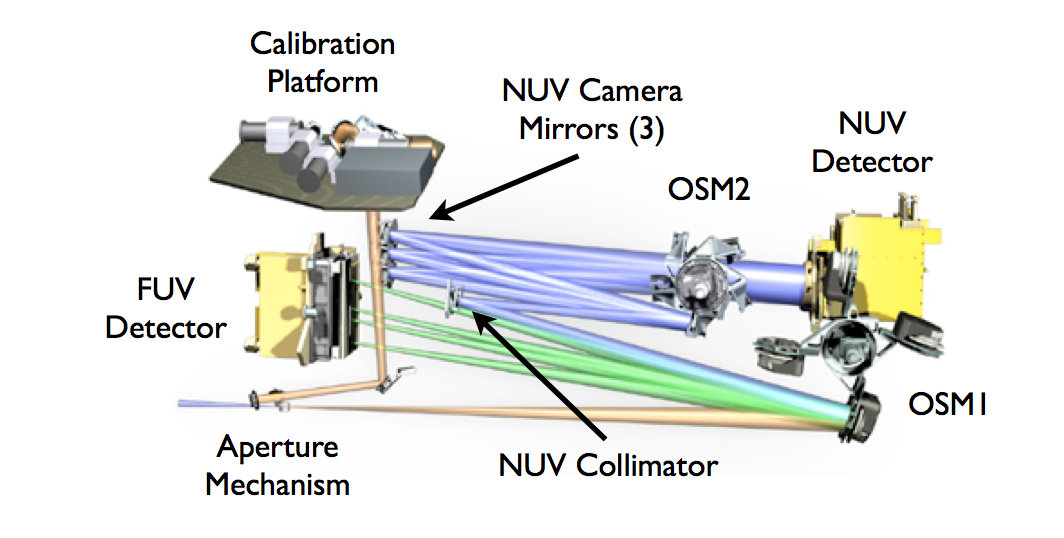
\includegraphics[width=\linewidth]{cos_optical.png}
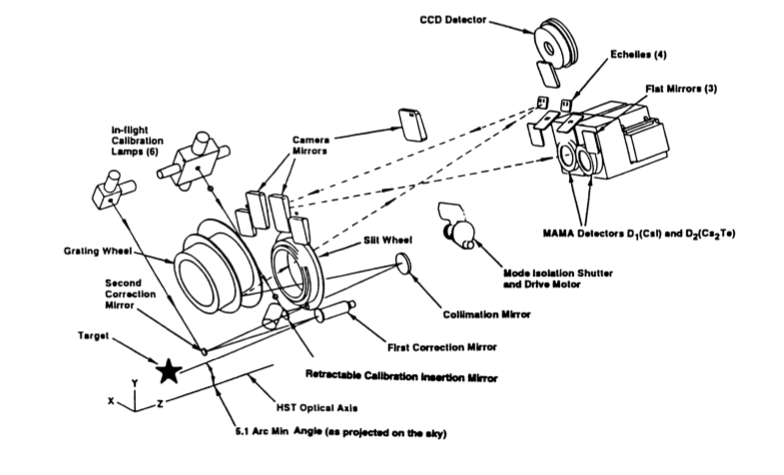
\includegraphics[width=\linewidth]{stis_optical.png}
\caption{Picture are the optical paths and elements of the two spectrographs on HST.  Though built on similar principles, the designs are very different.  \textit{(Top)} COS optical path.
\textit{(Bottom)} STIS optical path.}
\label{fig:x1d_2}
\end{minipage}
\end{figure}

%\begin{figure}[htbp!]
%\begin{center}
%\begin{minipage}[b]{.9\linewidth}
%\begin{center}
%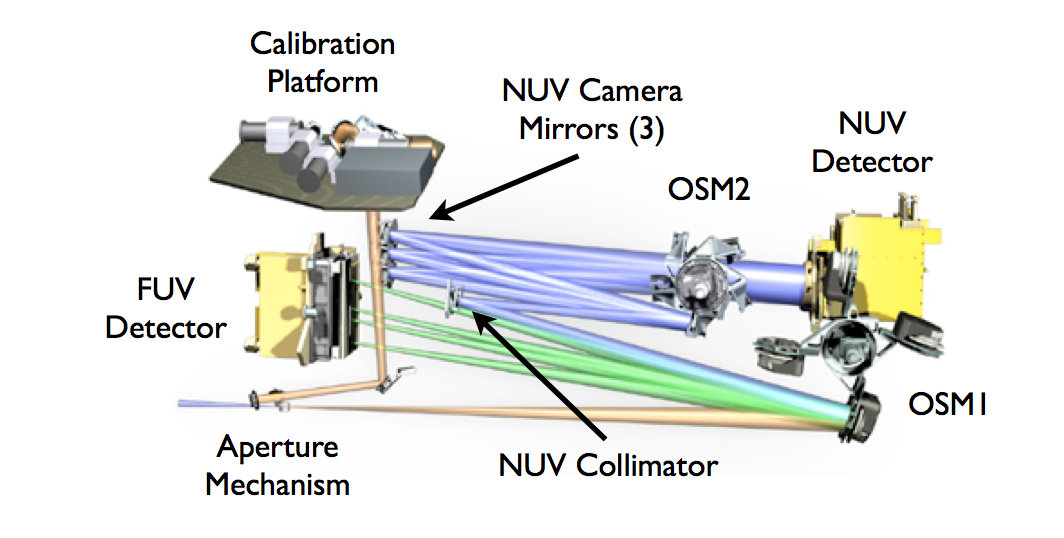
\includegraphics[width=\linewidth]{cos_optical.png}
%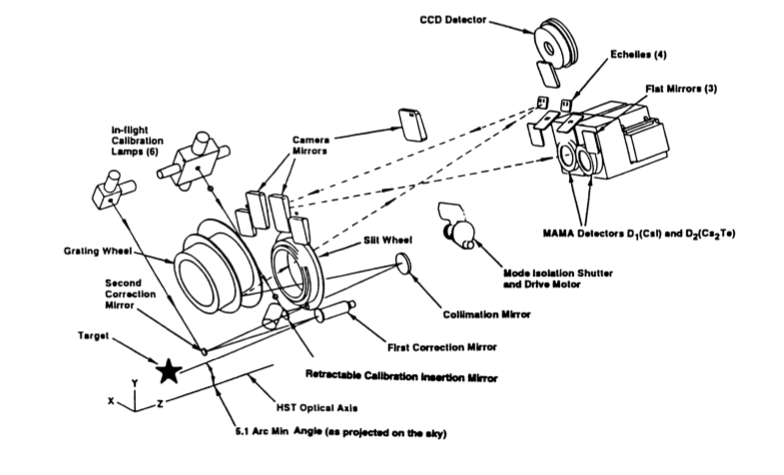
\includegraphics[width=\linewidth]{stis_optical.png}
%\caption{Picture are the optical paths and elements of the two spectrographs on HST.  Though built on similar principles, the designs are very different.  \textit{(Top)} COS optical path.
%\textit{(Bottom)} STIS optical path.}
%\label{fig:x1d_2}
%\end{center}
%\end{minipage}
%\end{center}
%\end{figure}

\section{Uses of Spectroscopy}
Spectroscopy is a very powerful tool used to probe the inner workings of distant objects.  It allows astronomers to measure chemical composition, redshifts, relative velocities, absorption systems, to name a few.

\section{Space-Based Spectroscopy}
\subsection{So many more wavelengths!}
Astronomy from the ground is inhibited by the Earth's atmosphere.   The elements that make up the atmosphere are only transparent to certain wavelength ranges, and so to observe any of the other ranges one must observe from space. See ~\ref{fig:atmo_trans}.

\begin{center}
\begin{figure}[htbp]
\begin{center}
% scale and angle values to be adjusted
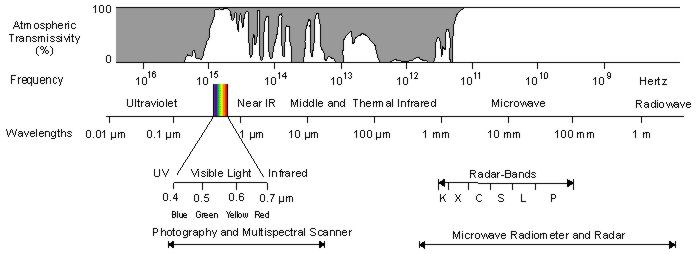
\includegraphics[scale=0.9, angle=0.0]{atmo_trans.jpg}
\caption{Atmospheric transmission with wavelength.  The low transmission at at many wavelengths, particularly UV and shorter, necessitates space based observations.}\label{fig:atmo_trans}
\end{center}
\end{figure}
\end{center}

\subsection{Airglow Lines}
The orbit of HST is close enough to earth to still encounter significant atmospheric effects.  One of the largest of these effects is the presence of emission lines caused by Earth's atmosphere.  The figures below show two of the more prominent lines, Lyman Alpha and Oxygen I.  Both of these features show variability on long and short timescales, with the former changing as HST passes through orbital day and night, and the latter changing as the solar cycle and the earth environment makes large scale changes to atmospheric size, density, etc.  

STIS has the ability to use small slits, and thus to remove much of the contamination from the airglow lines.  COS, however, has a fixed, large, aperture that cannot be used to filter out airglow.  Some filtering can still be done for COS data, but only by removing the part of the exposure that was taken during times of particularly strong airglow emission, such as orbital day. Strong airglow lines have led to the degradation of the COS FUV detector- to combat the damage done, the FUV spectra are periodically shifted up and down in XD (cross-dispersion) to expose on pristine portions of the detector.

\begin{figure}
\begin{minipage}[b]{0.5\linewidth}
\centering
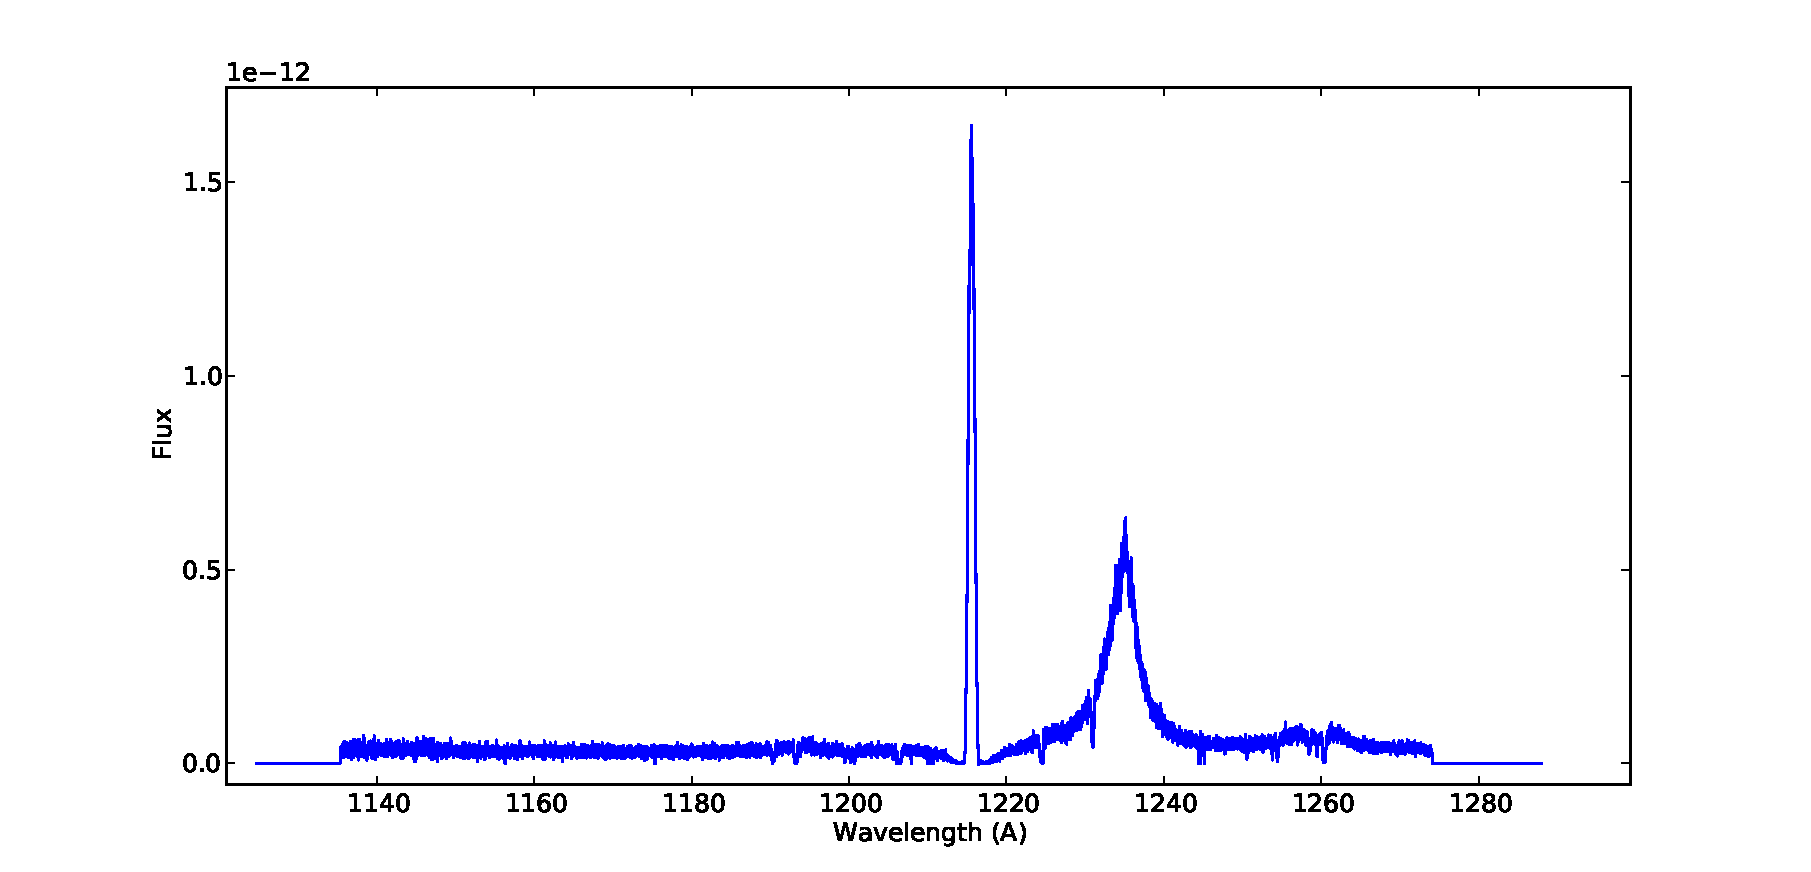
\includegraphics[width=\textwidth]{lya.pdf}
\caption{Geocoronal Lyman Alpha airglow is shown at 1216 \AA.}
\label{fig:geo1}
\end{minipage}
\hspace{0.5cm}
\begin{minipage}[b]{0.5\linewidth}
\centering
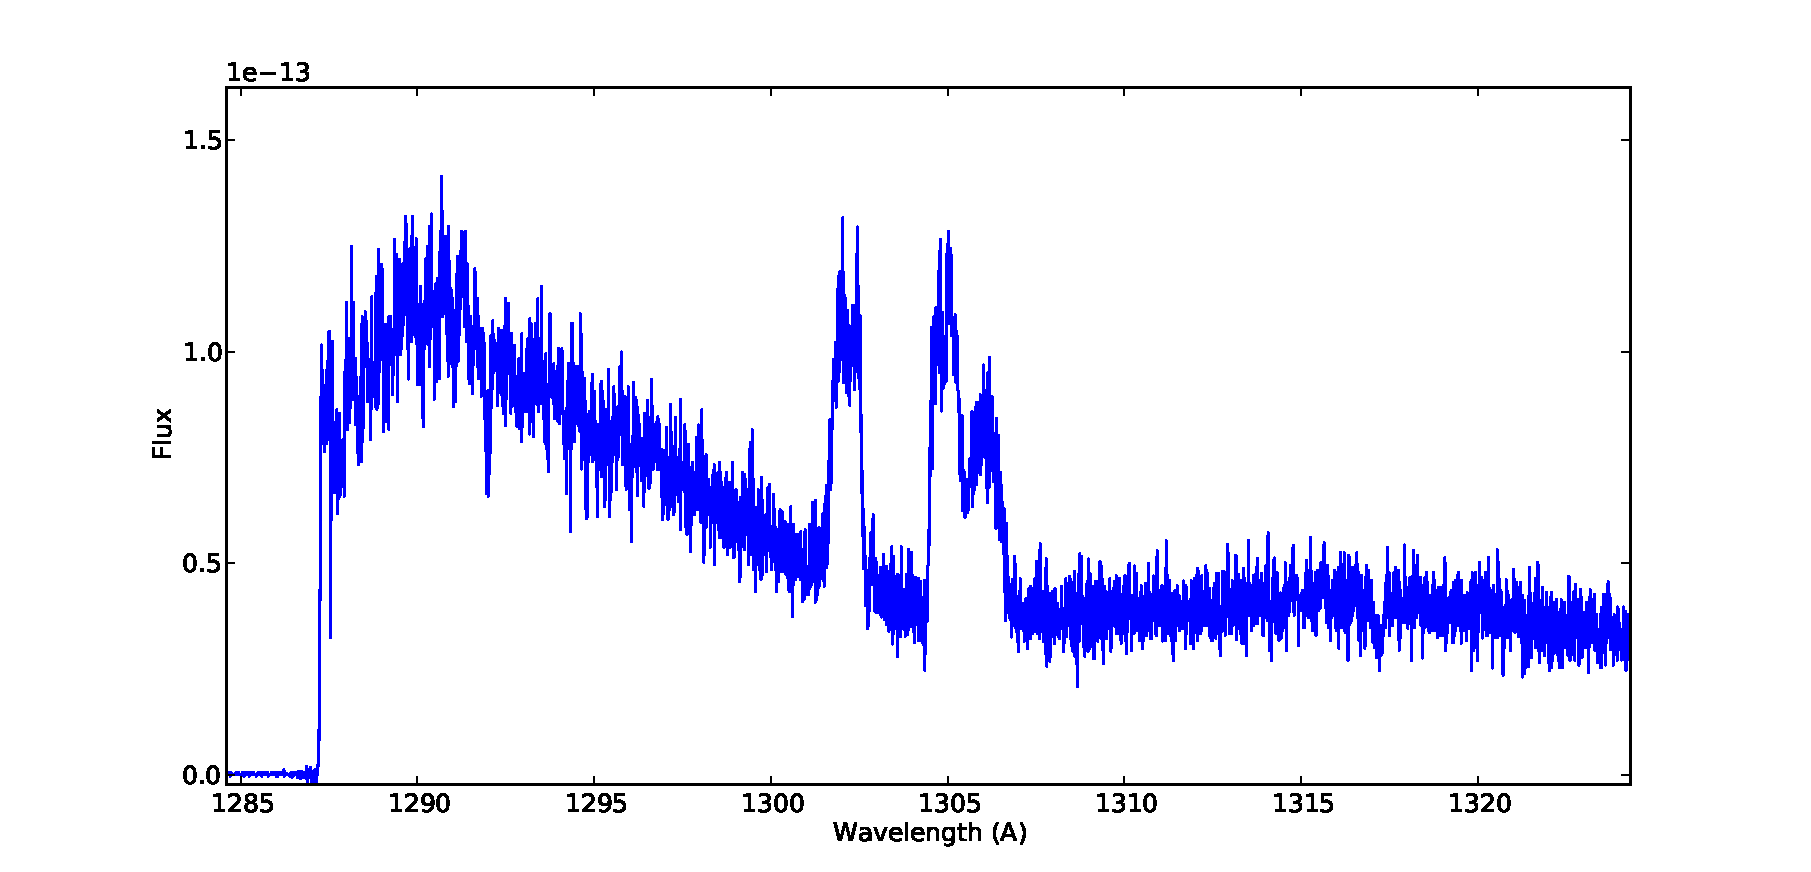
\includegraphics[width=\textwidth]{OIII.pdf}
\caption{Geocoronal Oxygen I airglow between 1300 and 1310 \AA.}
\label{fig:geo2}
\end{minipage}
\end{figure}


\subsection{UV Instrumentation}
Ultraviolet astronomy often requires different detectors than the typical Charged Couple Devices (CCDs).  HST employs two different kinds of UV detectors; Multi-Anode Microchannel Arrays (MAMAs), and an open face Microchannel Plate (MCP) with a Cross Delay Line Anode (XDL).  The MAMA detectors are employed in the FUV and NUV channels of STIS and the NUV channel of COS, while the XDL is only used in the COS FUV channel. 
%with the XDL only being used in the COS FUV channel.  

These detectors act very differently when compared to CCDs.  The most glaring difference is that these detectors are photon-counting devices.  This means that each incoming photon is uniquely observed by the instrument electronics.  This allows for some great flexibility, and great complexity, in processing of the data.  Data taken in TIME-TAG mode (default on COS, optional on some STIS modes), records the location and time of each photon event.  This means that data can later be screened not just in x,y location, but in time as well.  

UV detectors also experience an incredibly low background rate.  The FUV detector on COS, for example, has a mean dark count rate of $\sim 3.0x10^{-6} cnts/sec/pixel$.   To put this in perspective, in even very long exposures most pixels in the COS FUV detector do not have a single dark count.  

For a far more complete introduction to COS and STIS, along with any other HST instrument, please see that instrument's Instrument Handbook.

\subsection{Differences between COS and STIS}
While both of HST's spectrographs, COS and STIS, overlap in spectral range, there are still many unique advantages to each instrument that will dictate which is the best choice to achieve a program's goals. The FUV throughput, spectral resolution, and wavelength coverage of most COS modes is much higher than that of STIS. In addition, new "blue mode" COS configurations allow observations from the hydrogen Lyman limit (912 \AA) to Ly$\alpha$ (1216 \AA), far surpassing the wavelength range of STIS. The NUV capabilities of both instruments are comparable with the exception that it is easier to obtain broader NUV wavelength coverage with STIS. Generally speaking, STIS is better suited for observing extended sources than COS. Conversely, the COS instrument is optimized to observe point-source objects. The high-dispersion echelle modes of STIS offer resolving powers of up to $R \sim 200,000$. The significantly lower dark rates of COS make it a better choice when observing faint sources. 

Both detectors, however, share a number of features. Both instruments can observe using TIME-TAG mode, recording the time of each photon's arrival. Both COS and STIS MAMA detectors have brightness limits that ensure the safety of the instruments.